\section{RSA P/Q Mining}
\subsection{ In EDX finden Sie hierzu eine Aufgabe mit einer verschlüsselten Kommunikation. Entschlüs
seln Sie diese. Die entschlüsselten Informationen benötigen Sie in Übung 4.}
Bei dem RSA P/Q Mining wird das Phänomen ausgenutzt, dass es bei der Erstellung von RSA Schlüsseln dazu kommen kann, dass eine Primzahl teil von zwei öffentlichen Schlüsseln ist. Bei RSA besteht der Öffentliche Schlüssel aus dem Tuppel $(N,e)$, dabei wird $e$ gewählt und $N = p \cdot q$ mit $p,q$ prim. Wenn nun ein $N$ wie folgt berechnet wird:

$$N_1=p_1 \cdot q_1$$

und ein zweites 

$$N_2=p_1 \cdot q_2$$

Dann geht $p_1$ sowohl in die Berechnung von $N_1$ als auch in die Berechnung von $N_2$ ein. Somit ist $p_1$ ein Teiler von sowohl $N_1$ als auch von $N_2$. Wenn nun der ggT von $N_1$ und $N_2$ berechnet wird, dann gilt $ggT(N_1,N_2) = p_1$ somit kann eine der Beiden Primzahlen den Öffentlichen Schlüssels effizient berechnet werden. Damit ist es dann auch möglich $q$ zu berechnen mit: $$q_1 =\frac{N_1}{p_1}$$
Da so effizient die Primfaktoren von einem öffentlichen Schlüssel bestimmt werden können, kann damit auch schnell der private Schlüssel $d$ berechnet werden.
$$
d = e^{-1} mod (p_1 - 1) \cdot (q_1 -1)
$$
Für den anderen Öffentlichen Schlüssel funktioniert dies analog.
Auf diese Art und Weise ist es möglich aus zwei öffentlichen Schlüsseln die privaten Schlüssel zu berechnen, wenn eine Primzahl zufälligerweise als Primfaktor in beiden öffentlichen Schlüsseln vorhanden ist. 
Dieser Angriff kann nicht effizient oder gezielt angewendet werden. Es ist sehr unwahrscheinlich, dass in zwei öffentlichen Schlüsseln derselbe Primfaktor vorhanden ist. Allerdings ist es durchaus möglich den ggT von zwei öffentlichen Schlüsseln zu bestimmen, falls der ggT nicht 1 ist, ist der ggT direkt die Primzahl, welche als Faktor in beiden Ns enthalten ist.

\paragraph{Angriff}

Der Angriff wurde genau so umgesetzt. Es ist ein öffentlicher Schlüssel gegeben, von dem der private Schlüssel zu berechnen ist. Darüber hinaus ist eine verschlüsselte Nachricht gegeben, die dann anschließend entschlüsselt werden soll.

\begin{figure}[h]
\raggedright
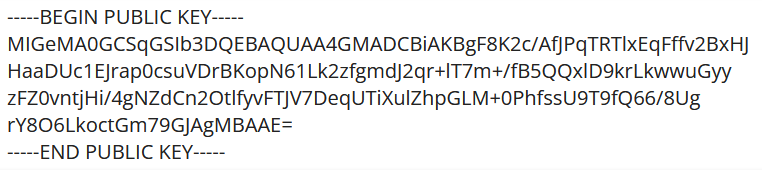
\includegraphics[width=0.7\textwidth]{img/ehup_ue3_pub_key.png}
\caption{Der gegebene Public Key}
\end{figure}

\begin{figure}[h]
\raggedright
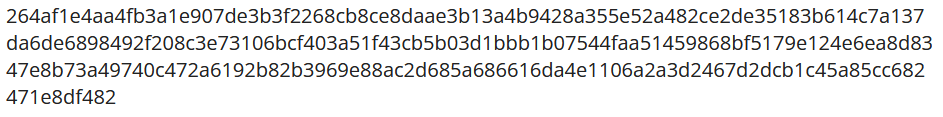
\includegraphics[width=0.7\textwidth]{img/ehup_ue3_priv_message.png}
\caption{Geheime Nachricht}
\end{figure}
Darüber hinaus sind auch 50 andere öffentliche Schlüssel im pem Format gegeben. Nun sei der gegebene öffentliche Schlüssel $N_1$ und die anderen $N_i$. Es wird im folgenden der ggT von $N_1$ und $N_i$ berechnet für alle gegeben Schlüssel. Wenn der ggT gleich 1 ist, dann ist es kein Treffer. Wenn der ggT nicht 1 ist, dann wurde $p_1$ gefunden und damit wird dann der private Schlüssel von $N_1$ berechnet.

Um das zu erreichen wurde ein Python Skript verwendet. In diesem wurde eine Methode namens mining definiert. Diese erhält die Ns und das e und gibt bei einem Treffer den geheimen Schlüssel von $N_1$ zurück.

\begin{figure}[h]
\raggedright
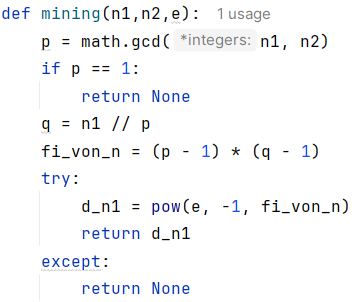
\includegraphics[width=0.7\textwidth]{img/ehup_mining_skript_v1.png}
\caption{Methode mining}
\end{figure}
Diese Methode wird nun für jeden gegeben öffentlichen Schlüssel ausgeführt und das Ergebnis erst mal für die Übersicht in der Konsole ausgegeben.

\begin{figure}[h]
\raggedright
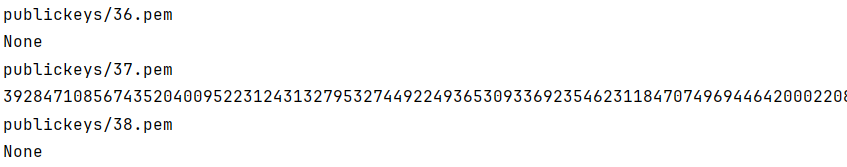
\includegraphics[width=0.7\textwidth]{img/ehup_ue3_ausgabe1.png}
\caption{Geheime Nachricht}
\end{figure}
In dieser Ausgabe wird jeweils der Name der Datei des zu testenden Schlüssels ausgegeben, sowei eine Ausgabe. Dabei wird None ausgegeben, falls kein Treffer vorliegt und der geheime Schlüssel bei einem Treffer. Es ist zu erkennen, dass in der Datei \texttt{37.pem} ein Treffer vorliegt. Gefunden wurde der geheime Schlüssel:
$$
\begin{aligned}
392847108567435204009522312431327953274492249365309336923546231184707496\\
944642000220807537351069389162386117042774266108845082525676854084662425\\
525675377329936511106161218412340079979544374189394100575353215643618410\\
583775546192217043211212172446378897226224722661765533424918159810410238\\
73593064057602439873
\end{aligned}
$$
Dieser geheime Schlüssel wurde anschließend in eine pem Datei geschrieben, um damit dann die geheime Nachricht entschlüsseln zu können. Diese lautet: \\ user815:8d93648f1ad5dc49002ef43b4a4685aa42cb3d9f87e861bc894f869713183f85

\begin{figure}[h]
\raggedright
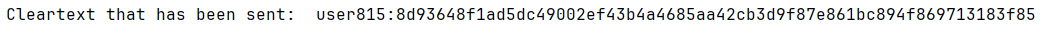
\includegraphics[width=1\textwidth]{img/ehup_ue3_ent_message.png}
\caption{Ausgabe der Entschlüsselung}
\end{figure}



\subsection{Überlegen Sie, wie es zu dem Phänomen kommt/kommen kann, das den Angriff erst ermöglicht!}
Zu diesem Phänomen kann es durch reinen Zufall kommen. Wenn ein RSA Schlüssel erstellt wird, dann werden zwei zufällige große Primzahlen gewählt. Aus diesen wird das $N$ für den öffentlichen Schlüssel berechnet. Wenn nun bei der Erstellung eines zweiten Schlüssels eine der beiden Primzahlen zufälligerweise wieder erezugt wird, dann kommt es dazu, dass $N_1$ und $N_2$ einen gemeinsamen Teiler haben. Dieser kann dann effizient berechnet werden. Es ist in der Praxis sehr unwahrscheinlich, dass es zu diesem Phänomen kommt, aber falls ein schlechter Zufallsgenerator verwendet wird, könnte es häufiger auftreten.

\subsection{Lassen sich SSH Verbindungen auf diese Weise aufbrechen? Welche Voraussetzungen wären dafür nötig, um dies zu ermöglichen?}
Ja auf diese Weise lassen sich auch SSH Verbindungen aufbrechen. Nötig wäre in diesem Fall auch, dass durch Zufall (z.B. durch schlechte Zufallszahlengeneratoren) eine Primzahl als Faktor in zwei öffentliche Schlüssel eingehen.

